\documentclass{article}
\usepackage{multicol}
\usepackage{amsmath,mathrsfs}
\usepackage{tikz}
\usetikzlibrary{arrows,shapes,chains}
\usepackage{flowchart}
\usepackage{xcolor}
\usepackage{setspace}
\usepackage{CJK}
\usepackage{geometry}
\usepackage{graphicx}
\usepackage{caption}
\usepackage{float,subfigure}
\geometry{a4paper,scale=0.8}
\usepackage[colorlinks,linkcolor=blue]{hyperref}
\hypersetup{CJKbookmarks=true}
\usepackage{parskip}
\setlength{\parindent}{0cm}

\begin{document}
\begin{spacing}{1.4}
\begin{CJK}{UTF8}{gbsn}
    \author{试卷来源:295356805(QQ群)\hspace{1cm}试卷提供:杳思思\hspace{1cm} 排版:回眸人}
    \title{2017华科824信号与系统}
    \maketitle
%\setlength{\parindent}{2em}

\section{填空题}
1、$cos2t+cos2\pi t$的平均功率是\underline{\hbox to 20mm{}}.
\vspace{1.5cm}

2、$\displaystyle\int_{-a}^{\infty}(t^2-6)\cdot u(2t-2)\cdot\delta(2t-6)dt$=\underline{\hbox to 20mm{}}.
\vspace{1.5cm}

3、$\displaystyle\int_{-\infty}^{\infty}sin2t\cdot\delta(t-1)dt$=\underline{\hbox to 20mm{}}.
\vspace{1.5cm}

4、$x[n]=2^n, n\leq 0$且$n$为偶数,则$X(e^{j\omega})$=\underline{\hbox to 20mm{}}.
\vspace{1.5cm}

5、$x[n]=\displaystyle\sum_{k=-\infty}^{\infty}(-1)^n\cdot\delta[n+k]$,则$X(z)$=\underline{\hbox to 20mm{}}.
\vspace{1.5cm}

6、$x(t)=y(t+1)-u(t-1)$,$y(t)=\displaystyle\int_{-\infty}^{t}x(\tau)d\tau$,则$X(s)$=\underline{\hbox to 20mm{}},收敛域为\underline{\hbox to 20mm{}},

\setlength{\parindent}{2em}
$Y(s)$=\underline{\hbox to 20mm{}},$Y(j\omega)$=\underline{\hbox to 20mm{}}.
\setlength{\parindent}{0em}

\pagebreak

\section{计算题}
1、$x(t)=\displaystyle\frac{(sin100t)^2}{\pi t^2}$通过如图系统,

\setlength{\parindent}{2em}
(1)求$X(j\omega), P(j\omega)$;
(2)求不混叠的$\Delta$最大值;
(3)若$\Delta=\frac{\pi}{100}$,求$X_p(j\omega)$;

(4)使$x_p(t)$通过一个低通滤波器$H(j\omega)=$
$\begin{cases}
1&,|\omega|<600 \vspace{-7pt} \\
0&,|\omega|>600
\end{cases}$,
假设此时$\Delta=\frac{\pi}{300}$,求$X_r(j\omega)$;

(5)设计一个系统,使$x_r(t)$通过后可以恢复$x(t)$.
\setlength{\parindent}{0em}
\vspace{-1.2cm}
\begin{figure}[H]
  \begin{minipage}[t]{0.5\linewidth}
    \centering
    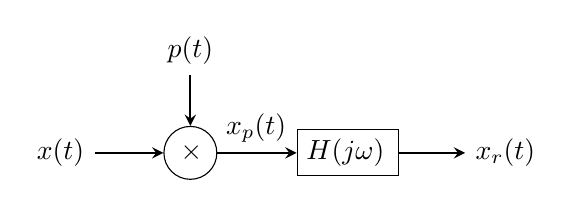
\begin{tikzpicture}[auto,node distance=20mm,>=stealth,thick]
      \tikzstyle{mul}=[circle,draw,thin,fill=white,text width=.7em]
      \tikzstyle{system}=[rectangle,draw,thin,fill=white,text width=3em]
      \node[mul](mul){$\times$};
      \node[left of=mul,xshift=10pt](x-in){$x(t)$};
      \node[above of=mul,yshift=-20pt](p-t){$p(t)$};
      \node[system,right of=mul](H-sys){$H(j\omega)$};
      \node[right of=H-sys](y-out){$x_r(t)$};
      \draw[->](x-in.east)--(mul.west);
      \draw[->](p-t.south)--(mul.north);
      \draw[->](mul.east)--(H-sys.west) node[above left]{$x_p(t)$};
      \draw[->](H-sys.east)--(y-out.west);
    \end{tikzpicture}
  \end{minipage}
  \begin{minipage}[t]{0.5\linewidth}
    \centering
    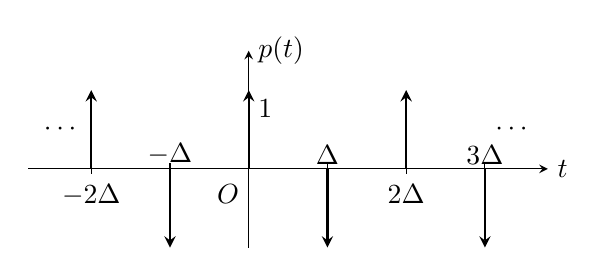
\begin{tikzpicture}
      \draw[->,>=stealth] (-2.8,0) -- (3.8,0) node[right] {$t$};
      \draw[->,>=stealth] (0,-1) -- (0,1.5) node[right] {$p(t)$};
      \draw[->,>=stealth,thick](0,0)--(0,1);
      \draw[->,>=stealth,thick](2,0)--(2,1);
      \draw[->,>=stealth,thick](-2,0)--(-2,1);
      \draw[->,>=stealth,thick](1,0)--(1,-1);
      \draw[->,>=stealth,thick](-1,0)--(-1,-1);
      \draw[->,>=stealth,thick](3,0)--(3,-1);
      \draw[shift={(3,0.5)},thick] (0pt,0pt) -- (0pt,0pt) node[right] {$\cdots$};
      \draw[shift={(-2,0.5)},thick] (0pt,0pt) -- (0pt,0pt) node[left] {$\cdots$};
      \draw[shift={(0,0)}] (0pt,2pt) -- (0pt,-2pt) node[below left] {$O$};
      \draw[shift={(0,1)}] (0pt,0pt) -- (0pt,0pt) node[below right] {$1$};
      \foreach \x/\xtext in {-2/-2\Delta, 2/2\Delta}
        \draw[shift={(\x,0)}] (0pt,2pt) -- (0pt,-2pt) node[below] {$\xtext$};
      \foreach \x/\xtext in {-1/-\Delta, 1/\Delta, 3/3\Delta}
        \draw[shift={(\x,0)}] (0pt,2pt) -- (0pt,-2pt) node[above] {$\xtext$};
    \end{tikzpicture}
  \end{minipage}
\end{figure}

\vspace{12cm}

2、题目不完整:
$h[n]-0.1h[n-1]-0.06h[n-2]$有限长,$u[n]$可和,$nu[n]$不可和;
\vspace{7cm}

\begin{minipage}{0.3\linewidth}
3、二输入二输出系统如图:

\setlength{\parindent}{2em}
(1)列状态方程;

(2)求$\phi(t)=e^{At}$;

(3)求$H(s)$.
\setlength{\parindent}{0em}
\end{minipage}
\begin{minipage}{0.7\textwidth}
\begin{figure}[H]
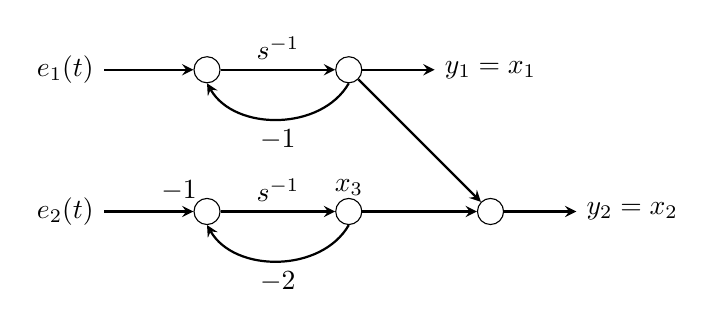
\begin{tikzpicture}[auto,node distance=18mm,>=stealth,thick]
\tikzstyle{unit}=[circle,draw,thin,fill=white,minimum width=.1pt, minimum height=.1pt]
  \node[](e1-in){$e_1(t)$};
  \node[unit,right of=e1-in](e1){};
  \node[unit,right of=e1](de1){};
  \node[right of=de1](y1){$y_1=x_1$};
  \node[below of=e1-in](e2-in){$e_2(t)$};
  \node[unit,right of=e2-in](e2){};
  \node[unit,right of=e2](de2){};
  \node[unit,right of=de2](x3){};
  \node[right of=x3](y2){$y_2=x_2$};
  \draw[->](e1-in)--(e1);
  \draw[->](e1.east) to[out=0,in=180] node{$s^{-1}$} (de1.west);
  \draw[->](de1.south) to[out=240,in=300] node{$-1$} (e1.south);
  \draw[->](de1)--(y1);
  \draw[->](e2-in)--(e2) node[above left]{$-1$};
  \draw[->](e2.east) to[out=0,in=180] node{$s^{-1}$} (de2.west) node[above,xshift=5pt,yshift=2pt]{$x_3$};
  \draw[->](de2.south) to[out=240,in=300] node{$-2$} (e2.south);
  \draw[->](de1)--(x3);
  \draw[->](de2)--(x3);
  \draw[->](x3)--(y2);
\end{tikzpicture}
\end{figure}
\end{minipage}
\vspace{7cm}

4、如图系统,输入$x(t)=(sint+cost)u(t)$时,输出$y(t)=\frac{1}{2}[sint+cost-e^{-t}]u(t)$,求:

\setlength{\parindent}{2em}
(1)$a,b,H(s)$;

(2)输入为$sint$时,求输出;

(3)若并联一个系统$h_1(t)$得到输出为$\delta(t)$,求$H_1(s)$和$h_1(t)$.
\setlength{\parindent}{0em}

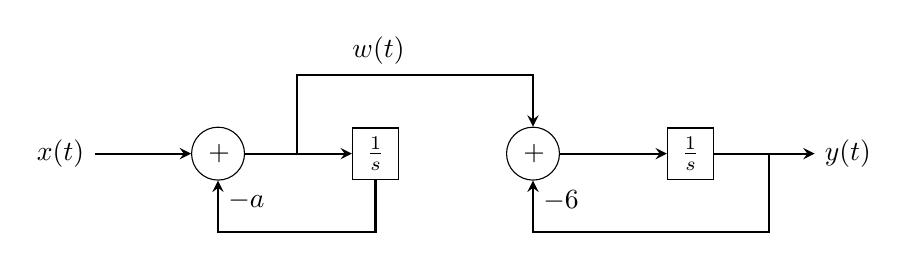
\begin{tikzpicture}[>=stealth,thick]
  \tikzstyle{add}=[circle,draw,thin,fill=white,text width=.7em]
  \tikzstyle{int}=[rectangle,draw,thin,fill=white,text width=1em,text centered]
  \node(x-in) at (0,0) []{$x(t)$};
  \node(add1) at (2,0) [add]{$+$};
  \coordinate(temp1) at (3,0)[]{};
  \node(int1) at (4,0) [int]{$\frac{1}{s}$};
  \node(add2) at (6,0) [add]{$+$};
  \node(int2) at (8,0) [int]{$\frac{1}{s}$};
  \coordinate(temp2) at (9,0) []{};
  \node(y-out) at (10,0) []{$y(t)$};
  \draw[->](x-in)--(add1);
  \draw[->](add1)--(int1);
  %\draw[->](int1.south) to[out=240,in=300,below] node{$-a$} (add1.south);
  \draw[->](int1.south)--(4,-1)--(2,-1)--(add1.south) node[below right]{$-a$};
  %\draw[->](temp1) to[out=60,in=120,above] node{$w(t)$} (add2.north west);
  \draw[->](temp1)--(3,1)--node[above left]{$w(t)$}(6,1)--(add2.north);
  \draw[->](add2)--(int2);
  \draw[->](int2)--(y-out);
  %\draw[->](temp2) to[out=270,in=300,below] node{$-6$} (add2.south);
  \draw[->](temp2)--(9,-1)--(6,-1)--(add2.south) node[below right]{$-6$};
\end{tikzpicture}




\end{CJK}
\end{spacing}
\end{document}
\grid
